\documentclass{report}
\usepackage[T1]{fontenc} % Fontes T1
\usepackage[utf8]{inputenc} % Input UTF8
\usepackage[backend=biber, style=ieee]{biblatex} % para usar bibliografia
\usepackage{csquotes}
\usepackage[portuguese]{babel} %Usar língua portuguesa
\usepackage{blindtext} % Gerar texto automaticamente
\usepackage[printonlyused]{acronym}
\usepackage{hyperref} % para autoref
\usepackage{graphicx}
\usepackage{indentfirst}
\bibliography{bibliografia}

\begin{document}
%%
% Definições
%
\def\titulo{Sonhos Lúcidos}
\def\data{Novembro 2022}
\def\autores{Martina Duque, Sofia Marrafa}
\def\autorescontactos{(113261) martina.duque18@ua.pt, (114591) sofiamarrafa@ua.pt}
\def\versao{VERSÃO 1}
\def\departamento{Dept. de Eletrónica, Telecomunicações e Informática}
\def\empresa{Universidade de Aveiro}
\def\logotipo{ua.pdf}
%
%%%%%% CAPA %%%%%%
%
\begin{titlepage}

\begin{center}
%
\vspace*{50mm}
%
{\Huge \titulo}\\ 
%
\vspace{10mm}
%
{\Large \empresa}\\
%
\vspace{10mm}
%
{\LARGE \autores}\\ 
%
\vspace{30mm}
%
\begin{figure}[h]
\center
\includegraphics{\logotipo}
\end{figure}
%
\vspace{30mm}
\end{center}
%
\begin{flushright}
\versao
\end{flushright}
\end{titlepage}

%%  Página de Título %%
\title{%
{\Huge\textbf{\titulo}}\\
{\Large \departamento\\ \empresa}
}
%
\author{%
    \autores \\
    \autorescontactos
}
%
\date{\today}
%
\maketitle

\pagenumbering{roman}

%%%%%% RESUMO %%%%%%
\begin{abstract}

Dormir bem é algo determinante no nosso dia a dia, sendo isso resultado de uma boa noite de descanso de sono, dando assim origem a sonhos, grande parte das vezes, de difícil recordação. Com a evolução da humanidade, a importância dos sonhos tem vindo a tomar outras proporções sendo que neles estão mensagens encriptadas do nosso inconsciente, revelando-nos alguns estados de espírito e até mesmo desejos.

O nosso cérebro passa por várias fases do sono. Quando se adormece inicia-se o sono leve de fase 1, seguido do sono leve de fase 2. Aí, começa o período de sono profundo, que é interrompido pelo sono leve de fase 2 e de seguida o de fase 1. Depois de estar na fase REM, o corpo volta novamente à fase 1 e repete todas as fases até voltar novamente à fase REM. Este ciclo vai-se repetindo ao longo de toda a noite, mas o tempo em sono REM vai aumentando em cada ciclo.

Os sonhos, o cerne deste projeto, podem ocorrer em todas as fases do sono e chegam a ocupar um total de duas horas por noite, mas geralmente são mais comuns no sono REM. Apesar de por vezes nem darmos conta disso, toda a gente sonha todas as noites. Esses sonhos podem ter a duração de poucos minutos a horas.

Para a ciência, o sonho é uma experiência, do inconsciente, durante nosso período de sono. Deste modo, vai ser explorado o que acontece no cérebro durante esses minutos de sonho, desde as suas bases neurobiológicas e as razões da sua existência até os seus benefícios, riscos e algumas curiosidades. 



%%%%%% Agradecimentos %%%%%%
% Segundo glisc deveria aparecer após conclusão...
\renewcommand{\abstractname}{Agradecimentos}
\begin{abstract}
Eventuais agradecimentos.
Comentar bloco caso não existam agradecimentos a fazer.
\end{abstract}

\tableofcontents
% \listoftables     % descomentar se necessário
% \listoffigures    % descomentar se necessário

%%%%%%%%%%%%%%%%%%%%%%%%%%%%%%%
\clearpage
\pagenumbering{arabic}

%%%%%%%%%%%%%%%%%%%%%%%%%%%%%%%%
\chapter{Introdução}
\label{chap.introducao}

É sabido que uma pessoa passa, em média, \textbf{um terço da sua vida a dormir} e \textbf{um quarto dela é passada a sonhar ativamente}, algo que é aprofundado no \autoref{chap.sonhos}. 

Dormir é algo vulgar, não só no ser humano mas em todo reino animal vertebrados, sendo que a sua privação é destruidora, não permitindo o regular funcionamento do sistema.

Posto isto, sujeitos à sua prática, o sono , composto por múltiplos estágios, caracteriza-se por ser um estado  de inconsciência onde cada pessoa pode ser “despertada” pelo seu subconsciente sendo que durante o mesmo,  o Sistema Nervoso central entra em intensa atividade levando-nos a sonhar.

Assim sendo, existem sonhos comuns a várias pessoas, tais como sonhar que se está a cair de um precipício, andar nu no meio da rua, fugir de um perigo, entre outros igualmente caricatos… 

De facto, é o nosso subconsciente que se reflete, mas sabia que é possível agir conscientemente durante um sonho? Parece improvável ou surreal, certo? De repente ser-se o argumentista de um filme. A estes dá-se o nome de sonhos lúcidos (\autoref{chap.ossonhoslúcidos}).

\chapter{Sonhos}
\label{chap.sonhos}

\section{O que os sonhos significam}
Independentemente da faixa etária, sonhar é algo comum a todos os seres humanos, sendo esta uma capacidade nata, onde todos são capazes de imaginar inconscientemente. Já muitos se questionaram as razões pelas quais conseguimos ter esta habilidade, e depois de alguns estudos sobre o tópico em questão, ainda não se conseguiu chegar a um consenso relativamente à terminologia de "sonho".
É interessante apercebemo-nos de como o nosso cérebro trabalha enquanto descansamos. Os sonhos podem decorrer durante \textbf{mais de duas horas}. Por isso, cientistas afirmam que uma pessoa pode passar até 6 anos de sua vida sonhando. Em média, uma pessoa sonha de \textbf{4 a 7 sonhos diferentes} em uma única noite. 


Nesta capacidade ainda por desmistificar, cerca de 95\% dos sonhos são completamente ignorados pelo nosso subconsciente e incompreensíveis, e como resultado disso, impossíveis de serem lembrados quando uma pessoa desperta. Contudo, sobra 5\% da conta, dado que é graças a essa pequena percentagem que nos questionamos pela sua existência, dado que apesar de mínima, ao acordar, as pessoas ficam memórias muito lúcidas e vívidas de algo que nem aconteceu, porém pareceu bastante real, guardando ainda na sua memória essas lembranças de algo que nunca aconteceu, sendo que nem sempre estes são memórias e histórias simples de se contar, tornando-se a maior parte das vezes em pequenos fragmentos de memória.
De forma geral, a caracterização que se atribui a um sonho é o facto de este corresponder a uma dada \textbf{sequência de fenómenos da mente que por norma ocorrem de forma voluntária durante o sono}. Enquanto isso, é possível verificar quando uma pessoa sonha através de algumas respostas fisiológicas criadas pelo organismo como consequência do estado de inconsciência comum, respostas estas como: movimentos rápidos dos olhos, perda da firmeza e força muscular, presença de excitação sexual, irregularização de batimentos cardíacos e a dessincronização das ondas cerebrais.
 
Entender o que é o sonho pode levar o sujeito a encontrar uma cura psicológica
Como já referido, \textbf{sonhar é um acontecimento natural de todo o ser o humano} e uma noite regular de sono provoca em média quatro a cinco períodos de sonhos, durante cerca de 20 minutos cada, podendo estes mais tarde não serem recordados, sendo que assim, é possível afirmar que de cada vez que uma pessoa dorme, este pessoa está a sonhar, contudo quando afirmarmos não termos sonhado, isso apenas acontece porque não nos recordamos do conteúdo do sonho.
A nível da saúde mental, os sonhos tem se vindo a revelar, com o passar do tempo de extrema importância, sendo que por detrás destes, apesar de surgirem de forma inconsciente, resultando dos mesmo diversas respostas às experiencias da vida consciente de cada um.

O sonhos tornam-se assim essenciais no restauro da saúde mental de cada um, \textbf{restablecendo um novo equibilibrio eletroquimico no cérebro}, prevenindo assim a sobcarga dos circuitos neuronais de cada um e, para além disso, faz com que sejam ainda proessados os acontecimentos diários, “armazenando” tudo o que é essencial e “processando” e até mesmo “eliminando” o restante.
Dado que o ato de sonhar é natural, este ato deve assim ser utilizado a favor da saude mental de cada um e por isso deve ser tido em contado como um sistema natural de cura psicológica. Para que isso aconteça, é apenas necessário saber trabalhar estes acontecimentos com técnicas especificas que contribuam para o autoconhecimento de cada um. Para além do mais, é importante resaltar a criativia inerte constante que acontece durante todo este processo, sendo que este visa uma uma constante busca por souções.
 
 	Com o passar dos anos, foi possível atribuir-se \textbf{três caminhos distintos} sobre a origem dos sonhos. O recordar da vida onírica é  um peça bastante importante para o autoconhecimento  a ser utilizado para ampliar a compreensão sobre a vida e sobre o que rodeia cada um. Isso traz uma resolução de problemas através de processos bastante  criativos. Durante uma sessão de psicanálise, as pessoas procurar chegar aos temas que estão bastante bem arrumados no seu inconsciente. Sendo que para Freud, “os sonhos são uma estrada para o inconsciente”.
  
Segundo  Freud, os sonhos podem surgir por três caminhos diferentes: estímulos sensoriais, restos diurnos e conteúdos inconscientes reprimidos·      
Estímulos sensoriais: O primeiro corresponde a todas as influências externas e internas que acontecem no decorrer da noite e que são assimiladas pelo inconsciente. 
Por exemplo: Uma pessoa sonha que está a passar uma noite no polo norte, onde está a passar muito frio e por isso está a viver uma experiência super desagradável, ou seja, quando acordar, provavelmente vai-se aperceber de que estava com os pés destapados durante uma noite fria de inverno. ·      
Restos diurnos: A segunda forma em que o sonho ocorre é “restos diurnos”.  Este é comum é pessoas que sempre tiveram habituados a uma vida de correria e muito agitada ou em que o que acontece ao seu redor é repentino, sendo que isso se poderá a vir a refletir em sonhos situações bastante semelhantes ao que  lhes foi acontecendo ao longo da vida.·      
Conteúdos inconscientes reprimidos - os sonhos que apresentam geralmente pensamentos, sentimentos e até  mesmo desejos, imersos no inconsciente, eram se refletir e manifestar nos sonhos.  
As distorções dos sonhos e os seus tipos de linguagens verbais

O tema que ocorre em cada sonho, está associado ao respetivo sono. Afinal, são os acontecimentos diarios e conflitos particulares que de forma consciente ou inconsciente afetam uma pessoa. Assim sendo, o sonho é uma bela ferramente para a resolução de problemas por desmistificar.
Algo curioso sobre tudo isto é o facto de todos os sonhos que conhecemos através de outros, não são mais nem menos que meros relatos, sendo que não temos a experiencia original de cada sonhador. Assim sendo, segundo Freud “É verdade que distorcemos os sonhos ao tentar reproduzi-los.” , sendo esse o mais natural processo da linguagem, sendo assim possivel saber que a linguagem verbal apresenta dois tipos de estruturas distintas : a superficial e a profunda. Ambas funcionam com universais linguisiticos denominados por genera generalização, distorção e eliminação.
 
A importância de repetir o processo para associação do paciente

Ao  fim do processo de revivier um sonho diversas vezes e de analisar esse destemunho,  é possível obter um quadro mais completo sobre o plano do sonho, sendo assim possivel realizar uma anãlise mais profunda e apropriada. Sendo este o método mais eficaz de analise, foi então este o método utilizado  por  Freud sendo que quando a repetição do relato divergi-se do anterior, seria então realizada um trabalho profundo de análise.A esse procedimento, Freud chamou de “interpretação fracionada do sonho.” 
 



Na psicanálise, correspondente à área científica que estuda a parte psíquica humana, isto é, investiga e preocupa-se em explicar o funcionamento da subjetividade humana e consequentemente tenta auxiliar no tratamento de alguns transtornos mentais, a concessão de sonho que existe está diretamente relacionada com o nosso inconsciente. Para além do mais, os sonhos apresentam uma diversidade imensa de naturezas, podendo estes serem melancólicos, assustadores, mágicos, de aventura, excitantes, entre outros.


Geralmente, algo que caracteriza os sonhos e que acaba por lhe dar interesse, é o facto de estes não poderem ser controlados por quem os está a ter, sendo que existe uma exceção, quando nos referimos a sonhos lúcidos, sonhos estes que serão descritos de seguida, mas que brevemente correspondem a sonhos onde o “sonhador” é autoconsciente dos acontecimentos. Uma particularidade dos sonhos, é a o facto de estes serem capazes de desenvolver um pensamento criativo e de certa forma alguma inspiração extra.


Segundo Freud, neurologista e pai da psicanálise, sendo uma das mais influentes figuras da psicologia, o sonho é a \textit{“principal via de acesso aos conteúdos que foram reprimidos pelo nosso inconsciente”}, isto é, quando se sonha, o que se encontra encoberto em nós, acaba por vir à tona, sendo que por vezes isso torna complicado definir a palavra sonho, tentando-se assim atribuir-se uma certa linha científica que justifique os acontecimentos.
 


\section{Quando sonhamos}
Posto isto, é permitido afirmar que os sonhos representam uma realidade externa afetando cada pessoa internamente. Estes são consequência da ativação cortical, ativação esta que ocorre na fase REM(rapid eye movement). A fase de REM acontece ao fim de três outras fases.
\begin{itemize}
\item \textbf{N1 ou NREM1 -} Esta é  a primeira fase, na qual é feita a transição entre o estado de desperto e adormecido e onde há queda na temperatura do corpo e uma desaceleração dos batimentos cardíacos, respiração e atividade cerebral
\item \textbf{N2 ou NREM 2 -}  Correspondente a cerca de 50\% do sono total, nesta fase o organismo “prepara-se” para atingir o estágio mais profundo do sono, relaxando assim os músculos e desacelerando a respiração.
\item \textbf{N3 ou NREM 3 -}  Nesta fase, será restaurado o sono. Permitindo assim que o organismo descanse devidamente e fortalecendo-lhe imunidade. Não é conveniente interromper este estágio de sono, podendo deixar a pessoa cerca de uma hora de atividade cerebral prejudicada.
\item \textbf{REM -} A fase de REM corresponde a paralisação temporal da musculatura, mas com a atividade intensa dos olhos e músculos da respiração. Esta é a fase mais difícil de acordar, sendo que o corpo fica “mole”, porém a atividade cerebral é intensa, permitindo assim sonhos mais vívidos e realistas. A intensidade da atividade cerebral é tamanha que é semelhante a quando o corpo está acordado.
\end{itemize}

\end{abstract}
\begin{figure}[h]
\center % Centra as imagens
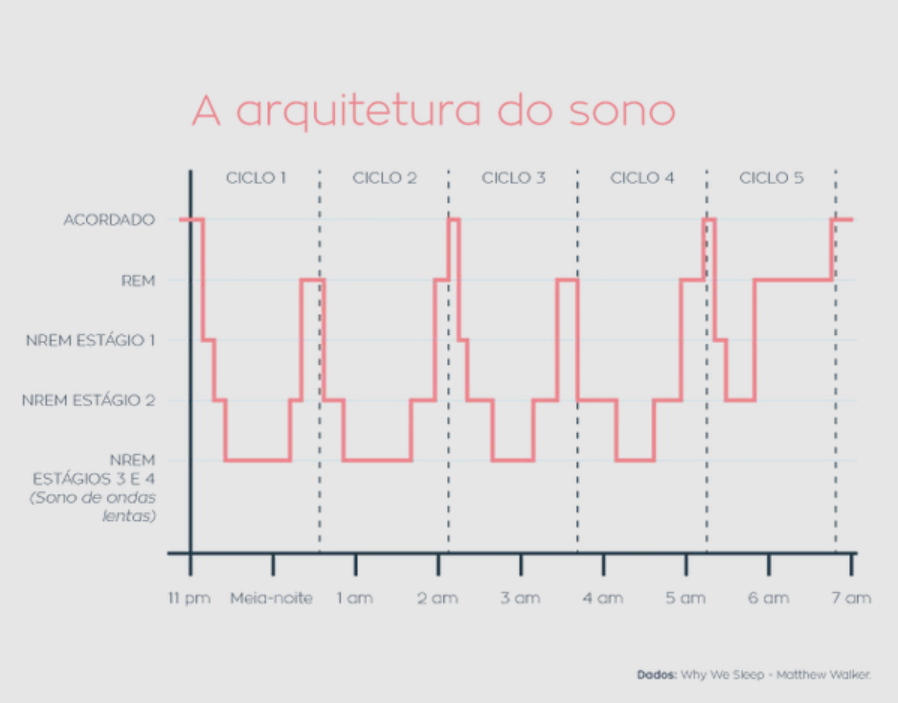
\includegraphics[width=100mm]{Arquitetura S.png}
\caption{Arquitetura do Sono}
\label{fig:sono}
\end{figure}
\section{Bases Neurobiológicas}
Geralmente, a caracterização mais comum que se dá a um sonho é o facto de este corresponder a uma dada sequência de fenómenos da mente que geralmente ocorrem de forma voluntária durante o período de sono. Enquanto se dorme, é possível verificar quando uma pessoa sonha através de algumas respostas fisiológicas criadas pelo organismo como consequência do estado de inconsciência comum, respostas estas como: movimentos rápidos dos olhos, perda da firmeza e força muscular, presença de excitação sexual, irregularização de batimentos cardíacos e a dessincronização das ondas cerebrais.

Bem, a razão pela qual nós sonhamos é que, durante o sono, o cérebro é praticamente totalmente ativado, tendo assim a necessidade de um fluxo de sangue duplicado, sendo apenas o “centro lógico”  a única parte que deixa de estar ativa no cérebro durante este processo.
A partir do momento em que isto acontece, os sonhos acontecem, sendo que para que estes não sejam exteriorizados pelo organismo, o cérebro envia sinais específicos à medula espinhal, paralisando assim os membros temporariamente, sendo que durante o sono o único movimento que geralmente ocorre é o dos olhos na fase REM.


Com isto, é importante frisar que em todas as fases de sono somos capazes de sonhar porém a quando em fase REM, os sonhos são mais ricos e imaginativos sendo que nas outras fases eles são geralmente mais simples e mutuamente difíceis de serem recordados. Apesar disso, na fase de REM, devido a baixíssimo nível de noradrenalina, hormona esta que é libertada para a corrente sanguínea, transmitindo sinais nervosos que ajudam a regular as funções cerebrais importantes tais como o sono, a atenção, o humor e a memória, quando despertamos devido à falta desta hormona, esta acaba-se por ser esquecida ao despertar, sendo que só somos capazes de os recordar caso despertemos 10 minutos após os termos. Tendo isto em consideração, os pesadelos são aqueles que fazem despertar com mais facilidade, devido ao facto das suas características intensas e assustadoras, levando assim a acordar repentinamente e com mais precipitação
\begin{figure}[h]
\center % Centra as imagens
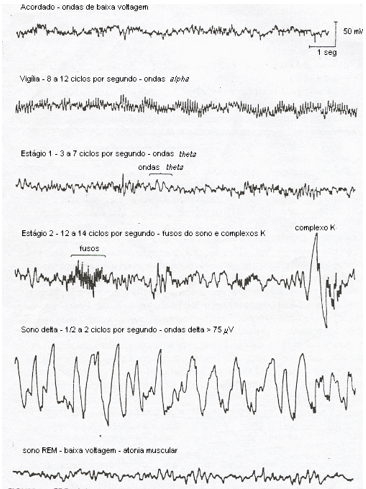
\includegraphics[width=80mm]{yyy.png}
\caption{fases do sono}
\label{fig:sono}
\end{figure}

\section{A importância dos sonhos para a psicologia}

Devido ao seu carácter inconsciente, dormir, e com isto fala-se de sonhar, pode-se revelar um ajudante dos problemas diários, dado que quando se sonha, o cérebro está constantemente a tentar solucionar os problemas que preocupam ao longo dos dias. Uma vez que os sonhos julgam-se ser o reflexo simbólico e significativo do que preocupa, assusta ou ostenta uma pessoa, acabando assim pelo maior parte das vezes as pessoas terem mais pesadelos, revelando-lhes os seus pesadelos e os problemas de autoconfiança pessoais.


Como já frisado, o processo de descanso realizado aquando uma pessoa dorme é essencial para o descanso pessoal de cada um, sendo que é nesse mesmo processo que cada um realiza uma seleção involuntária das suas memórias, sendo esta uma das razões para as quais é melhor dormir após se estudar ao invés de investir numa noite inteira de estudo.


\chapter{Os sonhos Lúcidos}
\label{chap.ossonhoslúcidos}
\section{O que são sonhos lúcidos}
O sono não é todo igual. Passamos por várias fases desde o sono mais superficial ao mais profundo, intercalados por períodos de sono REM, assim designado pelo movimento rápido de olhos característica desta fase: \textbf{Rapid Eye Movement(REM)} . Esses períodos vão-se tornando mais prolongados à medida que a noite avança, ocorrendo em maior percentagem pela manhã. Interessante este sono REM, está-se completamente paralisado, pode-se sonhar com uma ação, mas não a executar. A maior atividade do córtex pré-frontal que ocorre nesta fase é extremamente importante na consolidação de memórias para além de outras não menos importantes relacionadas com a mente. Durante os sonhos habituais (em REM), a atividade do córtex frontal e parietal está diminuída, o que faz com que a pessoa não consiga utilizar as memórias que utiliza quando acordado, não conseguindo por isso realizar uma auto análise do seu eu interno. Já nos sonhos lúcidos, há um aumento da atividade do córtex frontal e parietal, ao ponto do sonhador saber que está a dormir e a sonhar, conseguindo inclusive controlar o próprio sonho. Assim, o sonho lúcido resulta de uma memória nítida das informações facultadas pelo subconsciente.



\section{Benefícios terapeuticos e riscos}
Sonhos lúcidos, muitos já tiveram este tipo de sonho, mas nunca se aperceberam que podem ser um grande aliado não só porque abrem porta a grande diversão como também são benéficos para fins terapêuticos. Sabemos que o sonho é a chave para o nosso inconsciente, logo também é a chave para o acesso a memórias de que não nos recordamos. Na realidade, só se consegue resolver um problema se houver dados, correto?
De facto, o sonho organiza a memória com todo o tipo de informação que alguma vez já soubemos, por isso é possível que parte da sua função seja identificar associações e ligações que nunca descobriríamos acordados. Algumas das memórias que condicionam a nossa ação/ pensamento no presente foram esquecidas no passado. O sonho lúcido pode ser o mapa, nesse labirinto que é a memória.
 
Por exemplo, quando um menino vê ao fundo da rua um cãozinho com o olhar mais dócil deste mundo, e o seu amigo faz cem metros barreiras julgando ser um pitbull enfurecido. A origem deste comportamento poderá ter a ver com algum episódio do passado: terá sido mordida por um cão na infância? Terá o avô repetido vezes sem conta que o cão da vizinha é muito perigoso? A resposta estará lá… Como se descobrirá o acesso? Através do sonho lúcido!
Existe uma linha de pesquisa designada por imaginação motora, que sugere que ao imaginarmos os movimentos que queremos fazer, somos capazes de melhorar o desempenho dos mesmos na vida real, podendo beneficiar deficientes físicos ou atletas que queiram melhorar a sua performance.
Também os indivíduos que não nasceram cegos, mas perderam a visão por doença ou acidentes, possuem memória visual e podem sonhar com imagens. A quantidade e a forma dessas imagens irão depender da época em que perdeu a visão. Os sonhos lúcidos são assim um escape à escuridão, uma viagem “ilustrada”.
Assim, podendo controlar e alterar o sonho, através deles, é-se capaz de superar pesadelos, medos, resolver problemas, desenvolver capacidades, explorar a imaginação…
Como para tudo, ao desfrutar-se dos benefícios também se correm riscos. Alguns estudos defendem que passar pelo episódio com frequência pode provocar dificuldade para detetar a realidade. Isso poderia acontecer principalmente na hora de tentar lembrar se algo realmente foi ou não foi um sonho.
Além disso, a condição pode afetar a qualidade do sono. Não porque os sonhos tenham algum efeito negativo, mas porque você pode ficar tão viciado em viver em sonhos, que passa a dormir mais. Assim, o sono pode passar a sofrer influências, bem como a rotina.

\begin{figure}[h]
\center % Centra as imagens
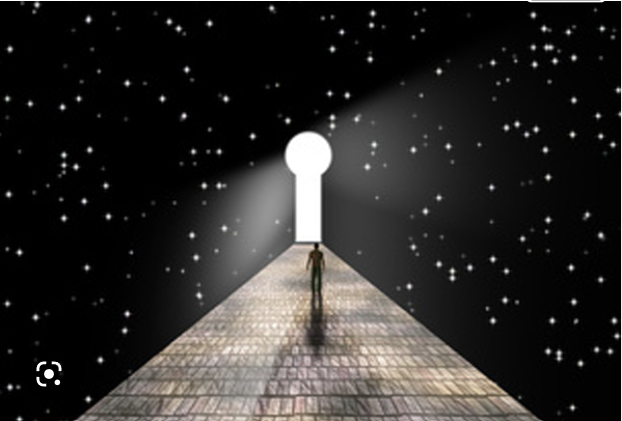
\includegraphics[width=100mm]{sonholucidooo.png}
\caption{Benefícios do sonho lúcido}
\label{fig:lucido}
\end{figure}


\section{Curiosidades}
Sonhos lúcidos tem muito que se lhe diga. Na verdade, acredita-se que os egípcios tinham os primeiros registos de sonhos lúcidos de sempre. Eles acreditavam que, por meio do Ba, estavam a viver dentro de seus sonhos. Assim, ele seria o primeiro exemplo de uma consciência além do plano real durante um sonho.
Outra curiosidade é que um estudo afirma que 20\% das pessoas passam por sonhos lúcidos mensalmente sendo que 50\% declarou ter passado pela experiência ao menos uma vez. Por outro lado, foi provado que crianças têm esses sonhos com maior frequência porque lidam mais com mais pesadelos, responsáveis por fases de lucidez durante o seu sono.
Curiosamente, participantes de um estudo realizado em 2006 confirmaram que o consumo diário de 250mg de vitamina B6 influenciou a lucidez durante o seu sonho, relatando serem mais vivos, mirabolantes e emocionantes. A \textbf{OMS} (organização mundial de saúde) recomenda que o consumo seja de 100 mg por dia. O consumo excessivo do suplemento pode gerar problemas como neuropatia sensorial, que gera dormência e perda de sensibilidade nas extremidades.



\section{Dicas de como ter um sonho lúcido}
A realidade é que é necessário dizer que os sonhos lúcidos são esporádicos e imprevisíveis. Apesar disso, foi cientificamente comprovado que os sonhos lúcidos podem ser induzidos, há cada vez mais pessoas que usam técnicas diferentes para entrar nos sonhos lúcidos como preferir.
O lado positivo é que qualquer cidadão pode aprender essas técnicas e utiliazá-las para entrar em sonhos lúcidos. Tal como qualquer músculo, o cérebro também consegue ser trabalhado, logo, através de algumas estratégias é possível sonhar-se de forma lúcida. Assim, é aconselhável acordar-se a meio da noite, aproximadamente 6 horas depois de se deitar ou, caso durma menos de 6 horas, acionar o despertador para um bocado mais cedo. Pode ir à casa de banho, correr em volta da cama, arrumar os tachos, como quiser…o que se pede é que se levante e fique em vigília durante 20 minutos… depois voltar a deitar-se. Enquanto retoma o sono é aconselhável pensar naquilo que quer sonhar para que a experiência tenha ainda melhores resultados! Este processo funciona, pois está-se a estimular o cérebro consciente num período em que há grande probabilidade de estarmos no sono REM, o sono dos sonhos. 
 
Para além disso, pode-se anotar o que é recordado do sonho. Não é grave se não se lembrar, o que é importante é criar o hábito. Com o tempo as memórias virão, este é um exercício para se lembrar deles… Durante o dia perguntar recorrentemente se está a sonhar também ajuda… Assim irá adquirir o hábito de o fazer durante o sonho, tornando-se cada vez mais fácil de entender que está a sonhar quando realmente estiver… Existem outras dicas complementares, como fazer um diário de sonhos.  Assim, cria-se um hábito de registo de sonhos, garantindo que se lembrará deles com mais frequência. Alguns pesquisadores também sugerem que deixar o telemóvel e outras telas de lado antes do sono pode ajudar. De facto, não é tarefa fácil alcançar a lucidez durante o sono mas como para tudo, com treino, dedicação e persistência é possível e recompensador.


A autodisciplina para a lucidez num sonho passa diretamente pela melhoria da capacidade de se testar a realidade várias vezes ao dia. Para além disso, é importante acrescentar que a consciência onírica desperta não provem apenas do treinamento da atenção e da memória, mas também do sentimento. A dúvida é um estado emocional de muito desconforto acompanhado normalmente por um espírito empreendedor e de vontade de descobrir, de conhecer. Quanto mais intenso for a curiosidade de sabermos se estamos a sonhar ou não, mais efetivos serão os testes de realidade. Tais fatos nos permitem averiguar se as pessoas mais emotivas são mais propensas ou não à lucidez e pode servir de guia e inspiração para estudos futuros.


\chapter{Conclusões}
\label{chap.conclusao}
Uma pessoa passa, num espaço de uma vida, um terço da sua vida a dormir e aproximadamente 6 anos só a sonhar, anos que podem ser de verdadeira terapia ou até mesmo de diversão. Afinal, há todo um mundo para descobrir, há uma nova canção para compor, novas gentes, novos credos, e tudo à distância de um Sonho Lúcido.
Alguns cientistas, entretanto, dizem que o discernimento de que se está a sonhar não é suficiente para que um sonho seja considerado lúcido e que é importante ultrapassarm este simples conceito, conferindo tal denominação apenas aos sonhos em que o sonhador apresenta controle consciente dos conteúdos que podem ser imaginados.
Na verdade é apenas na ciência que podemos dar os passos que o conhecimento corrente nos permite, jamais sabendo o que é aguardado durante esta caminhada. Afinal, não há consenso científico a respeito da essencia da razão pela qual existem  estes sonhos tão vívidos. Alguns modos sob os quais se apresentam baseiam-se no campo místico e estão fora do alcance do homem, da visão científica atual. Sabe-se, entretanto, que podem corromper os "alicerces" de nossas estruturas de realidade e levar à transcendência de todas as experiências formais. São factos que ainda dificultam o estabelecimento de uma definição acertiva.
Assim, este trabalho é um incentivo ao leitor a não passar seis anos da sua vida apenas a sonhar. 
Nas palavras de António Gedeão \emph{O sonho comanda a vida, sempre que um homem sonha, o mundo pula e avança}.




\chapter*{Contribuições dos autores}
Desde a pesquisa até ao produto final, o trabalho em equipa foi constante, pois as tarefas foram, justamente, distribuídas, tendo ambos os elementos cooperado na tentativa de apresentar o melhor trabalho possível.

Teste - \ac{md}  \ac{sm} 

\vspace{10pt}
\textbf{Indicar a percentagem de contribuição de cada autor.}\\

\autores : 50\%, 50\%\\

%%%%%%%%%%%%%%%%%%%%%%%%%%%%%%%%%
\chapter*{Acrónimos}
\begin{acronym}
\acro{ua}[UA]{Universidade de Aveiro}
\acro{leci}[LECI]{Licenciatura em Engenharia de Computadores e Informática}
\acro{glisc}[GLISC]{Grey Literature International Steering Committee}
\acro{md}[MD]{Martina Duque}
\acro{sm}[SM]{Sofia Marrafa}

 
\end{acronym}

%%%%%%%%%%%%%%%%%%%%%%%%%%%%%%%%%

\nocite{*}
\printbibliography



\end{document}